\documentclass[a4paper,12pt]{article}

% Packages for headers, footers, and general formatting
\usepackage[utf8]{inputenc} % Encoding
\usepackage{fancyhdr}       % Headers and footers
\usepackage{enumitem}       % For advanced lists
\usepackage[luatex]{hyperref}       % For clickable URLs, citations etc
\usepackage[usenames,dvipsnames]{color}%has to be called before tikz
\usepackage{tikz}
\usepackage{wrapfig}
\usepackage{adjustbox}
\usepackage{libertinus}
\usepackage{graphicx}
%\usepackage{setspace}
%\setstretch{1.25}
\usetikzlibrary{arrows.meta,graphs,graphdrawing,shapes.geometric}
\usegdlibrary{trees,circular,routing,}

\usepackage{color}
\usepackage[english,slovene]{babel} %language support
\usepackage{listings}
\usepackage[mode=buildnew]{standalone}

% Header and Footer Setup
\pagestyle{fancy}
\fancyhf{} % Clear all header and footer fields
%\fancyhead[R]{Your Header on the Left} 
%lstlistings popravek levega roba
%v glavi izmerim širino dveh majhnih številk in izračunam rob
\newlength{\MaxSizeOfLineNumbers}%
\settowidth{\MaxSizeOfLineNumbers}{\tiny 99}% Adjust to maximum number of lines
\addtolength{\MaxSizeOfLineNumbers}{2.5ex}%

\definecolor{lightgreen}{HTML}{CCFF99}
\fancyhead[C]{Optimizacija zaznave trkov v 2D}

\fancyfoot[C]{\thepage}
\setlength{\textwidth}{16cm}
\setlength{\oddsidemargin}{0cm}
\setlength{\headwidth}{\textwidth}

\lstset{
    numbers=left,
    numberstyle=\tiny,
    basicstyle=\ttfamily\small,
    keywordstyle=\color{violet},
    identifierstyle=\color{teal},
    extendedchars=true,
    xleftmargin=\MaxSizeOfLineNumbers,
    texcl=true,
    captionpos=b,
}

% \linespread{0.5}
% Begin Document
\begin{document}
\makeatletter
\addto\captionsslovene{
  % handle hyperref's autoref 
  \renewcommand\equationautorefname{enačba}%
  \renewcommand\footnoteautorefname{opomba}%
  \renewcommand\itemautorefname{alineja}%
  \renewcommand\figureautorefname{slika}%
  \renewcommand\tableautorefname{tabela}%
  \renewcommand\partautorefname{del}%
  \renewcommand\appendixautorefname{priloga}%
  \renewcommand\chapterautorefname{poglavje}%
  \renewcommand\sectionautorefname{razdelek}%
  \renewcommand\subsectionautorefname{podrazdelek}%
  \renewcommand\subsubsectionautorefname{podpodrazdelek-section}%
  \renewcommand\paragraphautorefname{odstavek}%
  \renewcommand\subparagraphautorefname{del odstavka}%
  \renewcommand\FancyVerbLineautorefname{vrstica}%
  \renewcommand\theoremautorefname{teorem}%
  \renewcommand\pageautorefname{stran}%
  % handle algorithm2e
  % \renewcommand{\listalgorithmcfname}{Seznam algoritmov}%
  % \renewcommand{\algorithmcfname}{Algoritem}%
  % \renewcommand{\algorithmautorefname}{\algorithmcfname}%
  % \renewcommand{\algorithmcflinename}{Vrstica}%
  % \renewcommand{\algocf@typo}{}%
  % \renewcommand{\@algocf@procname}{Procedura}%
  % \renewcommand{\@algocf@funcname}{Funkcija}%
  % \renewcommand{\procedureautorefname}{\@algocf@procname}%
  % \renewcommand{\functionautorefname}{\@algocf@funcname}%
  % \renewcommand{\algocf@languagechoosen}{slovene}%
  % handle lstlistings
  \renewcommand{\lstlistingname}{Izpis}%
}
\makeatother
 %slovene captions for hyperref and algorithm2e
% Title Page
\begin{titlepage}
    \title{\Huge Optimizacija zaznave trkov v 2D}
    \date{}
    \maketitle
    \renewcommand{\headrulewidth}{0cm}
    \fancyhf{}
    \fancyfoot[L]{Mentor: Klemen Bajec\\Avtor: \author{Klemen Javoršek}}
    \fancyfoot[R]{Gimnazija Vič\\Ljubljana, 2024/2025}
    \thispagestyle{fancy}
    %\setcounter{page}{1} 
\end{titlepage}
\selectlanguage{slovene}
\graphicspath{snips}
% Table of Contents
\newpage
\quad
\thispagestyle{empty}
\newpage
\tableofcontents
\newpage
\section*{Povzetek}
V raziskavi smo implementirali dvodimenzionalen fizikalni simulator. 
Da bi omogočili gladko delovanje pri velikem številu objektov, smo uporabili podatkovno strukturo
za optimizacijo zaznave trkov: k-d drevo. Simulator smo napisali v programskem jeziku C, izvaja pa se enonitno.

V nalogi raziskujemo, kako lahko z različnimi nastavitvami drevesa vplivamo na hitrost simulacije
in ugotavljamo, kateri deli programa porabijo največ izvajalnega časa. Natančno opišemo tudi podatkovne
strukture in nekaj zanimivih podrobnosti osnovnih funkcij simulatorja.

Preučimo tudi, kako na hitrost simulacije vpliva velikost sektorjev k-d drevesa, kakšen je vpliv
reciklaže sektorjev ter kakšen je vpliv značilnosti objektov, ki jih simuliramo. V raziskavi smo
dobili veliko podatkov, ki jih bomo v prihodnje lahko uporabili za optimiziranje našega simulatorja.
\section*{Ključne besede}
simulator, zaznava trkov, k-d drevo, optimizacija, programiranje, programski jezik C, fizikalne simulacije,
logična drevesa, računalniške igre
\newpage
\section{Uvod}

V računalništvu je zaznava trkov problem, pri katerem ugotavljamo, katera telesa ali objekti
v določenem sistemu se stikajo ali sekajo. Nanj pogosto naletimo v fizikalnih simulacijah,
računalniških igrah, robotiki, programski opremi za računalniško podprt razvoj (CAD) in tudi drugje.

Če moramo najti vse pare objektov, ki se sekajo, moramo primerjati vse objekte med sabo.
Najpreprostejši algoritem za zaznavanje trkov bi primerjal vsak objekt z vsakim drugim objektom. Časovna
zahtevnost takega algoritma bi bila zelo slaba: $O(n^2)$, kjer je $n$ število objektov v sistemu.

Omejujoči volumni so skupina oblik, ki jih algoritmi za zaznavanje trkov uporabljajo namesto dejanskih objektov.
Ker so objekti pogosto zapletenih oblik, je preverjanje parov objektov lažje izvajati z omejujočimi volumni.
Taki algoritmi trk natančno preverijo šele takrat, ko sta dva omejujoča volumna trčila. Na ta način se izognejo
časovno zahtevnemu primerjanju objektov kompleksnih oblik.

Ker je naš simulator namenjen le raziskovanju, lahko celoten postopek poenostavimo: vsi objekti so v obliki
kroga, kar pomeni, da sploh ne potrebujemo omejujočih volumnov. Na ta način še vedno lahko raziskujemo
obnašanje takega sistema, hkrati pa odstranimo veliko nepotrebnih komplikacij.

Glavni cilj, ki si ga zastavljamo pri zaznavi trkov, je, da se čim bolje izognemo kvadratni zahtevnosti
rešitve problema. To lahko dosežemo na več načinov, ki pa imajo vsi eno skupno lastnost -- objekte 
primerjajo samo s tistimi objekti, ki so jim blizu. Predstavili bomo nekaj načinov razdeljevanja prostora,
ki se najpogosteje uporabljajo.

Pristop \textit{pometi in poreži} je pristop, pri katerem omejujoče volumne projiciramo na vse koordinatne osi prostora. Če se vse projekcije
dveh volumnov med sabo sekajo, volumna upoštevamo kot kandidata za bolj natančno zaznavanje trkov. Da jih lahko med sabo učinkovito
primerjamo, morajo biti projekcije v sortiranem seznamu. Zaradi zahtevnosti sortiranja projekcij je ta pristop
učinkovit samo takrat, ko se objekti ne premikajo prehitro.

\textit{Zaznavanje s pomočjo homogene mreže} je način zaznave trkov, pri katerem ustvarimo mrežo, ki pokriva prostor, v katerem
so objekti. Vsak objekt vstavimo v vse celice mreže, ki se z njim prekrivajo. Razmerje med velikostjo mreže in velikostjo
objektov zelo močno vpliva na učinkovitost pristopa. V idealnem primeru so objekti približno enako veliki ali manjši kot
je velika celica v mreži. Težave se lahko pojavijo, kadar imamo zelo velik prostor ali zelo
hitro premikajoče se objekte. Če algoritma ne implementiramo zelo pazljivo, lahko postane prostorsko ali časovno potraten.

\textit{Algoritmi z drevesnimi strukturami} so algoritmi, ki za izboljšanje učinkovitosti uporabljajo drevesne strukture.
Naloga drevesnih struktur je, da simulacijo razdelijo na majhne dele. Objekt, za katerega moramo zaznati trke,
lahko potem primerjamo samo z objekti v delih drevesa, ki so mu v simulaciji fizično blizu. Časovna učinkovitost 
iskanja po takih drevesih je ponavadi {\small$\log_{p \cdot r}(n)$}, kjer je $p$ število neposrednih potomcev vsakega vozlišča,
$r$ število objektov, ki so v vsakem področju shranjeni, $n$ pa število objektov v celotni simulaciji. 

Nekaj popularnih dreves~\cite{weller_brief_2013} so drevesa BVH (\textit{Bounding volume hierarchy -- hierarhija omejujočih volumnov}),
drevesi \textit{štiriško drevo} in \textit{osmiško drevo}, drevo BSP (\textit{Binary space partitioning tree -- dvojiško drevo za razdeljevanje prostora}) in njegov posebni primer, \textit{k-d ali k-di\-men\-zi\-o\-nal\-no drevo}. 

\begin{itemize}
    \item Hierarhija omejujočih volumnov je drevo, sestavljeno iz omejujočih volumnov, ki vsebujejo
    druge omejujoče volumne. Obstaja več variacij tega drevesa, ki uporabljajo različne vrste omejujočih volumnov
    in različne algoritme za grajenje dreves ter iskanje, vstavljanje in brisanje objektov.
    \item Štiriško drevo je drevo, ki prostor simulacije rekurzivno razdeljuje na štiri enake dele. Uporabno je,
    ker je zelo preprosto in zato časovno učinkovito.~\cite{re_analysis_1985}
    \item Osmiško drevo je verzija štiriškega drevesa, ki razdeljuje 3-D prostor. To počne na zelo podoben način kot štiriško drevo, ampak
    prostor namesto na 4 razdeli na 8 enakih delov.~\cite{schnabel_octree-based_2006}
    \item Drevo BSP je iskalno drevo, ki dvodimenzionalen prostor rekurzivno razdeljuje s pomočjo razdelitvenih "hiperravnin",
    torej prostorov, ki so eno dimenzijo manjši od prostora, ki ga drevo razdeljuje. V 2D prostoru je hiperravnina premica,
    v 3D prostoru kar navadna ravnina, v 4D prostoru je pa to že 3D prostor. Hiperravnine so lahko orientirane
    poljubno, kar omogoči, da se oblika vozlišč v drevesu z globino vedno bolje približuje oblikam objektov v drevesu.~\cite{chin_iii5_1995}\cite{mehta_handbook_2018}

    \item K-dimenzionalno drevo je drevo, ki prostor razdeljuje s pomočjo ravnin. Objekti na eni strani vsake razdelitvene
    ravnine spadajo v enega neposrednega potomca, ostali pa v drugega. Drevo je narejeno za prostor s poljubnim številom dimenzij,
    zato se orientacija ravnin spreminja, ko potujemo po drevesu. Ravnine so vzporedne koordinatnim osem, torej je v
    $k$-dimenzionalnem drevesu $k$ različnih orientacij razdelitvene ravnine.~\cite{ramasubramanian_generalized_1989}
    
\end{itemize}

\begin{figure}
    \centering
    \adjustbox{max width=0.6\textwidth, fbox}{
        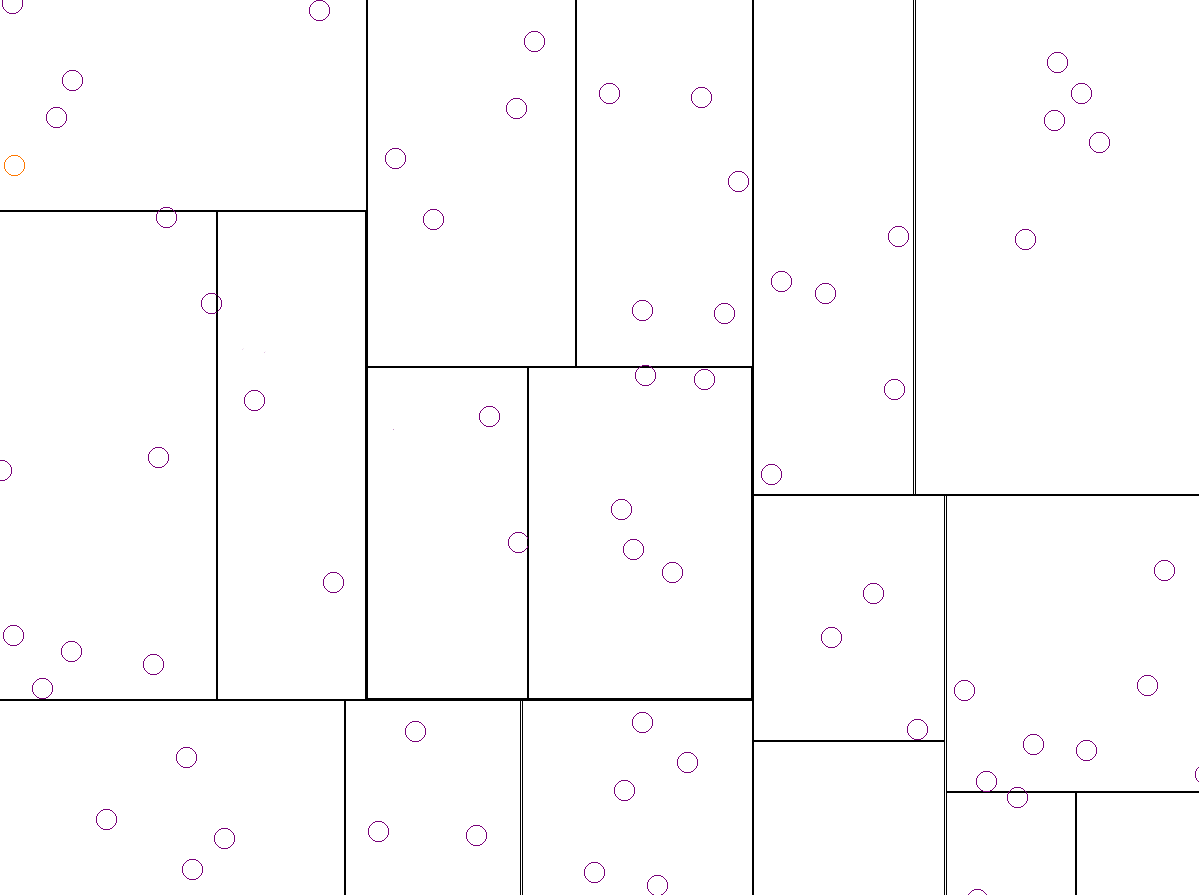
\includegraphics{screenshot1}
    }
    \caption{Prikaz dela simulacije s pomočjo knjižnice SDL2; prikazane so meje vozlišč drevesa in objekti}
\end{figure}



Odločili smo se, da bomo naše objekte organizirali s pomočjo k-dimenzionalnega drevesa.\@ Na osnovi naše implementacije drevesa
smo zgradili simulator v dveh dimenzijah in ga opremili s kodo, ki meri porabo časa simulatorja in njegovih
komponent.

Simulator je sestavljen iz štirih zaporedno izvedenih postopkov:
\begin{enumerate}
    \item Zaznava trkov
    \item Popravljanje vektorjev hitrosti objektov in njihovega položaja v drevesu
    \item Premikanje objektov
    \item Reciklaža praznih ali skoraj praznih vozlišč
\end{enumerate}

V nadaljevanju naloge bomo opisali, kako je k-d drevo zapisano v pomnilniku, kako delujejo različni
algoritmi v tem drevesu, in kako delujejo pomožne funkcije, ki ne izvajajo zaznave trkov. Po tem opisu
bomo raziskovali, kako spreminjanje lastnosti drevesa vpliva na hitrost delovanja našega simulatorja,
ter iz tega izpeljali zaključke, ki bi lahko v prihodnosti privedli do bolje zasnovanega simulatorja.

Celotna izvorna koda simulatorja je objavljena na spletni strani Github: https://github.com/telvivace/firja/tree/mr25
\newpage
\subsection{Hipoteze}
\begin{enumerate}
    \item Podatki bodo pokazali, da lahko določimo optimalno število objektov v vozlišču drevesa, pri katerem
je simulator najbolj učinkovit.
    \item Koncentracija objektov v simulaciji močno vpliva na hitrost simuliranja.
    \item S pomočjo reciklaže vozlišč se lahko izognemo temu, da bi morali ponovno graditi drevo. 
    \item Razporeditev objektov v prostoru ima velik vpliv na učinkovitost postopka reciklaže.
\end{enumerate}

\newpage


\section{Fizikalni simulator}

\begin{wrapfigure}{r}{0.4\textwidth}
    
    \vspace{0.2cm}
    \centering

    \tikz[>={Stealth[round,sep]}]
      \graph[simple necklace layout, necklace routing, grow'=down, node sep=1em,
              nodes={draw,rounded corners,rectangle,align=flush left,text width=3cm,scale=0.7}]
      {
        Zaznava trkov -> Popravki na osnovi zaznanih trkov -> Premikanje objektov -> Optimizacija drevesa -> Zaznava trkov
      };
    
    \vspace{1cm}
\end{wrapfigure}

Simulator, ki smo ga implementirali, deluje v ciklih. V vsakem ciklu se izvede več korakov: zaznava trkov, upoštevanje
zaznanih trkov, premikanje objektov v simulaciji in optimizacija k-d drevesa. Funkcije, ki imajo
povezavo s fizičnim stanjem v simulaciji, morajo biti neodvisne od vrstnega reda izvajanja operacij na objektih.
Zato, na primer, ne moremo vseh korakov izvajati hkrati. Tako izvajanje bi ustvarilo nepredvidljive rezultate,
ki so odvisni od vrstnega reda, v katerem procesiramo objekte v simulaciji. Ker moramo zagotoviti koherenco med
vsemi pristopi k zaznavi trkov in simulaciji, si tega ne moremo privoščiti. Koraki se iz tega razloga izvajajo
zaporedno, kar nam zagotovi, da se bo simulacija pri enakih začetnih pogojih vedno enako iztekla.


\begin{itemize}
    \item Zaznava trkov je najpomembnejši korak, zaradi katerega sploh potrebujemo k-d drevo. V tem koraku rekurzivno
    obiščemo vsako vozlišče v drevesu in za vsak objekt zaznamo trke. Zaznane trke zapišemo v objekte.
    \item V naslednjem koraku prav tako obiščemo vsa vozlišča in upoštevamo zaznane trke. To pomeni, da popravimo vektorje hitrosti
    vseh objektov, ki so bili vpleteni v trk. Poleg tega opravimo tudi nekaj ostalih nalog kot je zagotavljanje,
    da so objekti v pravilnih vozliščih, in da objekti ostanejo znotraj meje simulacije. Ena od teh nalog je tudi,
    da prepoznamo vozlišča, ki so (skoraj) prazna in jih damo v čakalno vrsto za optimizacijo.
    \item Po popravkih se morajo objekti tudi premakniti. Za to poskrbi tretji korak, kjer ponovno obiščemo vse objekte in
    jih premaknemo v skladu z njihovimi vektorji hitrosti.
    \item Zadnji korak je optimizacija drevesa. V tem koraku pregledamo čakalno vrsto za optimizacijo in iz drevesa izločimo
    prazna ali skoraj prazna vozlišča. Na ta način ohranjamo učinkovitost simulatorja v primeru prostorsko nehomogene
    simulacije.
\end{itemize}

Taka ureditev simulatorja omogoči koherenco, a hkrati lahko vidimo tudi, da v vsakem ciklu vsak objekt obiščemo 3-krat.
Sodobni računalniki so omejeni predvsem s hitrostjo in zamikom branja in pisanja po pomnilniku in predpomnilniku. 
To pomeni, da je tak način obiskovanja objektov zelo potraten in potreben optimizacije. Na žalost bi bilo zelo zahtevno
implementirati simulator, ki vse objekte obišče le enkrat na cikel in hkrati ohrani koherenco, a bi verjetno z veliko truda
in statusnimi zastavicami na objektih to bilo mogoče. Po drugi strani je pa zmanjšati število ogledov vseh objektov iz 3 na 2 veliko
lažje. V naslednjih poglavjih si bomo ogledali, kako bi se to dalo narediti, ter bolj natančno opisali, kako deluje vsak korak.

\newpage
\section{Drevo objektov}

\begin{wrapfigure}{r}{0.4\textwidth}
    
    \vspace{0.2cm}
    \centering

    \tikz[tree layout, grow'=down, level distance=11mm, sibling distance=3mm,
          nodes={draw,fill=cyan!40,circle,inner sep=2pt, scale=0.6}
    ]
    \node{NULL}
    child {node {NULL}
      child {node {NULL}
      }
      child {node[fill=red!50]{0x7F...}
        child{node[draw, rectangle, fill=white]{[... , ...]}}
      }
    }
    child {node {NULL}
      child {node {NULL}}
      child {node {NULL}}
    };
    \caption{Drevo z vozliščem z objekti}%
    \label{fig:drevo_z_buf}

\end{wrapfigure}

Naša implementacija fizikalnega simulatorja za pospeševanje zaznave trkov uporablja k-d drevo.
Drevo se razdeljuje po premicah, ki so vzporedne koordinatnima osema.

Drevo je sestavljeno iz vozlišč, ki so v jeziku C~\cite{gustedt_modern_2024} implementirana kot strukture (gl.\ izpis \ref{node_struct}).
Za preprostejšo uporabo je drevo povezano navz\-dol in navzgor -- vsako vozlišče ima kazalce na svojega
neposrednega prednika in oba neposredna potomca.
Razdeljevanje poteka s pomočjo dveh spremenljivk: smeri razdelitve (po osi $x$ ali osi $y$), ter
pozicije razdelitve (primer: 1334,5). Na tak način lahko funkcije, ki se spuščajo po drevesu,
učinkovito določijo naslednje vozlišče, ki ga bodo obiskale. Objekti so v
drevesu shranjeni le v vozliščih, ki nimajo potomcev, to so končna vozlišča ali listi.
V vsakem vozlišču je tudi \lstinline|buf|, kazalec na del pomnilnika, v katerem so shranjeni objekti.
Ena od praktičnih lastnosti kazalca je, da pokaže, ali je vozlišče končno vozlišče.

\begin{lstlisting}[caption={Struktura vozlišča}, label=node_struct, language=C]
struct treeNode {
    struct treeNode* left;
    struct treeNode* right;
    struct treeSplit split;
//  vsebina strukture treeSplit:
//      unsigned isx;
//      double value;
    struct treeNode* up;
    object* buf; // NULL -> list
    uint64_t places; //bitmask: prazen = 1, zaseden = 0
    rect_llhh bindrect; //okvir, ki ga zaseda vozlišče
    unsigned level; // kako globoko v drevesu je vozlišče
    uint16_t flags;
    uint16_t optindex;
};
\end{lstlisting}


V vozlišču je shranjen tudi pravokotnik \lstinline|bindrect|: ta opisuje površino, ki jo pokriva vozlišče v simulaciji.
Z njegovo pomočjo lahko ugotovimo, ali je treba objekt premestiti v drugo vozlišče.
Pomemben del vsakega vozlišča je bitna maska \lstinline|places|, ki označuje lokacijo vsakega objekta v kosu
pomnilnika, kjer so shranjeni objekti. Tako lahko z eno bitno operacijo preverimo tudi, ali je v vozlišču
preveč objektov in ali ga je zato treba razdeliti. Z procesorskim ukazom \lstinline|popcount| lahko objekte tudi
hitro preštejemo. Poleg tega je v strukturi tudi bitna maska \lstinline|flags|, ki omogoča označevanje vozlišča,
če ima vozlišče poseben status.

\subsection{Iskanje po drevesu}

Hitro iskanje objektov je ključnega pomena za dobro delovanje našega simulatorja.
To je razlog, da uporabljamo k-d drevo, ki nam omogoča, da objekt hitro najdemo le s
pomočjo njegovih koordinat.

Obstajata dve vrsti iskanja:
iskanje točke (objekta) ter iskanje območja (pravokotnika). Iskanje točke je pomembno za
vstavljanje in ponovno vstavljanje objektov v drevo, iskanje območja pa za zaznavo trkov.


Iskanje točke na izpisu \ref{find_parent_node} sicer ni rekurzivno, a smo v rekurzijo primorani
pri iskanju območja, in sicer zaradi tega, ker se lahko območje, ki ga iščemo, prekriva z več različnimi vozlišči.
Temu algoritmu ni treba biti rekurziven, saj vedno izbere samo eno pot po drevesu, zato lahko namesto
rekurzije uporabimo kar zanko \lstinline[language=C]{for}.

\begin{samepage}
Iskanje v drevesu poteka na preprost način (gl.\ tudi izpis~\ref{find_parent_node}):
    \begin{enumerate}
        \item Začnemo pri korenu drevesa.
        \item Preverimo, ali ima trenutno vozlišče kazalec na objekte.
        \item Če kazalec ima, potem je to končno vozlišče. Vrnemo kazalec na vozlišče.
        \item Če kazalca nima:
        \begin{itemize}
            \item Preverimo, po kateri koordinati ($x$,$y$) je vozlišče razdeljeno.
            \item Razdelitev primerjamo z relevantno koordinato objekta.
            \item Glede na primerjavo se premaknemo na levega ali desnega potomca.
            \item Vrnemo se na korak 2.
        \end{itemize}    
    \end{enumerate}
\end{samepage}

Za pravilno delovanje simulatorja je poleg iskanja točke pomembno tudi iskanje pravokotnika. Algoritem je zelo podoben
iskanju točke. Razlika med algoritmoma je, da moramo pri iskanju pravokotnika
ob vsaki razdelitvi vozlišča preveriti, ali se pravokotnik prekriva s premico, ki deli vozlišče. V tem
primeru je treba rekurzivno poklicati funkcijo na obeh neposrednih potomcih, saj oba vsebujeta del pravokotnika. Zaradi takih
situacij se pogosto zgodi, da iskanje pravokotnika vrne kazalce na več vozlišč, zato moramo računati na poljubno število
rezultatov iskanja.

\newpage

\begin{lstlisting}[float, caption={Iskanje vozlišča, ki vsebuje objekt}, label=find_parent_node, language=C]
    treeNode* tree_findParentNode(objTree* tree, object* obj){
        treeNode* currentNode = tree->root;
        while(1) {
            if(currentNode->buf) return currentNode; // smo na dnu
            switch(currentNode->split.isx) {
                case 1: // x split
                    if(obj->x < currentNode->split.value){
                        currentNode = currentNode->left;
                    }
                    else {
                        currentNode = currentNode->right;
                    }
                    break;
                case 0: // y split
                    if(obj->y < currentNode->split.value){
                        currentNode = currentNode->left;
                    }
                    else {
                        currentNode = currentNode->right;
                    }
            }
        }
    }
\end{lstlisting}


Algoritem za iskanje pravokotnika v drevesu lahko opišemo na naslednji način:
\begin{samepage}
    \begin{enumerate}
        \item Preverimo, ali ima trenutno vozlišče kazalec na pomnilnik z objekti (torej je končno vozlišče).
        \item Če kazalec ima, potem je to končno vozlišče. Ta kazalec dodamo na seznam rezultatov.
        \item Če kazalca nima:
        \begin{itemize}
            \item Preverimo, po kateri koordinati ($x$,$y$) je vozlišče razdeljeno.
            \item Razdelitev primerjamo z našim iskalnim pravokotnikom.
            \item Če razdelilna premica seka pravokotnik, dvakrat pokličemo sami sebe.
            Pokličemo se z obema deloma pravokotnika.
        \end{itemize}
    \end{enumerate}
\end{samepage}

\newpage
\subsection{Grajenje drevesa}

\begin{wrapfigure}{r}{0.6\textwidth}
    \centering
    \includestandalone{snips/unbal_tree}
    \caption{Neuravnoteženo drevo, če vstavljamo objekte, urejene po koordinatah}%
    \label{fig:drevo_unbal}
\end{wrapfigure}

Za grajenje dreves obstaja veliko pristopov. Cilj vsakega pristopa je ponavadi čimbolj
uravnoteženo drevo. Večina jih je prilagojenih na to, da moramo v drevo vstavljati že vnaprej
narejene objekte, ki jih želimo organizirati. Včasih so takšni objekti na urejeni po položaju v prostoru,
kar lahko povzroča težave. Ker želimo z našim simulatorjem le raziskovati, lahko izberemo zelo 
preprost, a učinkovit način ustvarjanja uravnoteženega drevesa: vstavljanje naključnih objektov.

Vstavljanje naključno izbranih objektov v drevo poskrbi, da bo novonastalo drevo dobro uravnovešeno.
Če bi objekte vstavljali urejene po lokaciji, bi nastalo slabo zgrajeno, neuravnoteženo drevo, kot je
drevo na sliki~\ref{fig:drevo_unbal}.



Če hočemo objekt vstaviti v drevo, moramo najprej najti pravo vozlišče, nato preveriti,
ali je slučajno polno, in v tem primeru vozlišču dodati dva potomca ter jima razdeliti objekte.
(O tem bomo več povedali pod naslovom Deljenje vozlišč)

Objekti so v svojem kosu pomnilnika razporejeni na nepredvidljiv način, in sicer zato, ker so se nekateri
zaradi svoje pozicije zunaj pravokotnika, ki ga pokriva njihovo vozlišče, morali prestaviti v drugo vozlišče.

\subsubsection{Zapis objektov v pomnilniku}
Vsako končno vozlišče ima kazalec na kos pomnilnika, v katerega lahko spravimo
točno določeno maksimalno število objektov. Da se izognemo nepotrebnim, časovno potratnim dostopom
do teh objektov, moramo nekaj informacij o njih zapisati že v strukturo vozlišča.

Podatek, ali je določeno mesto polno ali prazno, lahko zapišemo z enim bitom. Ker je objektov več,
moramo bite sestaviti v bitno masko. V ta namen uporabljamo \lstinline|uint64_t places|, ki je v strukturi 
\lstinline|treeNode|. S pomočjo takega 64-bitnega števila lahko spremljamo zasedenost kosa pomnilnika 
do največ 64 objektov, kar je več kot dovolj za naše potrebe.

\newpage
Nekaj osnovnih operacij~\cite{gcc_documentation} je opisanih v izpisu~\ref{bitmask_examples}:
\begin{lstlisting}[caption={Uporaba bitne maske za objekte}, label=bitmask_examples, language=C]
    // preveri, ali je na indeksu N objekt
    !(node->places & (1UL << N))

    // preveri, ali je cel kos pomnilnika popisan.
    // OBJBUFSIZE je največje število objektov.
    !(node->places & ((1UL << OBJBUFSIZE) -- 1)) 

    // indeks prvega prostega mesta
    __builtin_ctzll__(node->places)

    // indeks prvega objekta
    __builtin_ctzll__(~node->places)

    // koliko je objektov
    __builtin_popcountl__(~node->places)

    // zapišemo, da je prostor N zaseden
    node->places &= ~(1UL << N)

    // zapišemo, da je prostor N prost
    node->places |= (1UL << N)

\end{lstlisting}


\subsubsection{Alokacija pomnilnika}

\looseness=-2
Ker ta program lahko zahteva veliko pomnilniškega prostora, je smiselno, da namesto sistemskega
alokatorja \lstinline|malloc(), calloc(), ...| uporabimo lasten, preprostejši alokator.
Ker se mora sistemski alokator spoprijemati s težavami, kot so: fragmentacija pomnilnika, sproščanje
prej alociranih delov pomnilnika in mnoge druge težave, mora zelo pazljivo ravnati z alokacijami in
izvajati vrsto operacij, ki nam jih sicer znotraj konteksta našega simulatorja
ne bi bilo treba izvajati. Zato je smiselno, da implementiramo zelo preprost linearni alokator, ki nam lahko služi kot orodje
za spremljanje količine porabljenega pomnilnika, predvsem pa zelo pospeši alokacijo novih struktur.
Implementirali smo linearni alokator, ki v zakulisju alocira velike kose pomnilnika s pomočjo
funkcije \lstinline|calloc()|, koščke teh alokacij pa potem daje funkcijam, ki pomnilnik uporabljajo.
Ker naš simulator vse alocirane kose pomnilnika ponovno uporabi, nam na primer sploh ni treba implementirati
funkcije \lstinline|free()|, ki jo sistemski alokator mora zagotoviti. Alocirani bloki pomnilnika znotraj našega
alokatorja si vedno sledijo eden za drugim, brez lukenj. Če bi želeli podatke serializirati take, kot so,
bi vzeli alokatorjev seznam vseh večjih kosov pomnilnika, jih zlepili skupaj in zapisali v datoteko.
To je veliko preprosteje, kot če bi imeli nešteto majhnih sistemskih alokacij.

\subsection{Deljenje vozlišč}
Ko število objektov v določenem vozlišču doseže maksimalno vrednost, moramo to vozlišče
razdeliti. Ta postopek zahteva alokacijo struktur za dve novi vozlišči in alokacijo vsaj enega novega
kosa pomnilnika za objekte. Poleg tega je treba vsaj en del objektov prestaviti v drugo vozlišče.
Proces deljenja vozlišča je torej relativno časovno potraten postopek, ki si ga ne želimo izvajati
preveč pogosto. Na splošno skušamo zmanjšati število operacij s pomnilnikom, in tako prihranimo veliko
časa.

Preden se poglobimo v podrobnosti deljenja vozlišč, ne smemo pozabiti, da iskalne funkcije preverjajo,
ali je vozlišče končno, s pomočjo kazalca \lstinline|buf|, ki nastavljen le pri končnih vozliščih. 
Zato moramo vozlišču, ki ga delimo, kazalec nastaviti na \lstinline[language=C]|(void*)0|.

Cilj deljenja je, da pod vozliščem ustvarimo dva potomca, ki imata vsak svoj del objektov. Med deljenjem
je treba prilagoditi tudi bitne maske \lstinline|places| vozlišča in obeh potomcev.

Nedognan način deljenja vozlišča bi bil lahko:
\begin{itemize}
    \item Alociramo dve novi vozlišči, ki bosta potomca.
    \item Alociramo dva nova kosa pomnilnika za njune objekte.
    \item Izračunamo mediano x ali y koordinat objektov (odvisno od lokacije v drevesu).
    \item Zapišemo mediano v \lstinline|split| originalnega vozlišča.
    \item Na podlagi mediane razdelimo objekte med oba potomca. Med kopiranjem
    posodabljamo bitno masko \lstinline|places| obeh potomcev.
    \item Prvotnemu vozlišču odstranimo kos pomnilnika z objekti.
\end{itemize}
Ta način zahteva dve alokaciji in eno odstranitev kosov pomnilnika. Poleg tega moramo
vse objekte prekopirati iz prvotnega kosa pomnilnika v kosa pomnilnika obeh potomcev,
kar zahteva ravno toliko operacij, kot je maksimalno število objektov v vozlišču.

Bolj dognan način deljenja vozlišč pa bi potekal tako:
\begin{itemize}
    \item Alociramo dve novi vozlišči, ki bosta potomca.
    \item Alociramo en nov kos pomnilnika za objekte.
    \item Izračunamo mediano x ali y koordinat objektov (odvisno od lokacije v drevesu).
    \item Na podlagi mediane prestavimo $ \frac{n}{2}$ objektov iz prvotnega kosa pomnilnika
    v drugi kos pomnilnika. Med prestavljanjem posodabljamo \lstinline|places| vozlišča in njegovega potomca.
    \item Iz prvotnega vozlišča prestavimo kazalec, ki kaže na njegov kos pomnilnika, na njegovega potomca.
    \item Iz prvotnega vozlišča prekopiramo bitno masko \lstinline|places| v potomca, ki je podedoval tudi pomnilnik.
\end{itemize}
Drugi način zahteva eno alokacijo in samo $\frac{n}{2}$ operacij premikanja. To pomeni, da je postopek
dvakrat hitrejši, kar je zelo dobrodošla sprememba.

Sama funkcija za deljenje vozlišč je zelo dolga, zato si bomo ogledali samo najpomembnejši
del, to je prestavljanje objektov. Še nekaj podatkov v zvezi s kodo: spremenljivka \lstinline|parent|
je vozlišče, ki ga cepimo, spremenljivka \lstinline|dest| pa je vozlišče, v katero kopiramo objekte.
Naloga vrstice 8 je, da standardizira operacijo za obe mogoči razdelitvi: $x$ in $y$. Strojna koda, v
katero se ta vrstica prevede, je zelo podobna, kot če bi napisali \lstinline|parent->buf[i].x|, a s pomembno razliko, da izbira
polja \lstinline|x| ali \lstinline|y| v strukturi ni vnaprej določena med prevajanjem.

\begin{lstlisting}[caption={Razdeljevanje objektov med potomcema}, label=balance_buffers, language=C]
if(parent->split.isx) 
    coordoffset = offsetof(object, x);
else 
    coordoffset = offsetof(object, y);
unsigned destwritten = 0;
for(unsigned i = 0; i < OBJBUFSIZE; i++){
    //first value is the x or y field of the i-th struct in buf
    if(*(double*)( (char*)&(parent->buf[i]) + coordoffset )
     > parent->split.value)
        {
        memcpy(dest->buf+destwritten, parent->buf+i, sizeof(object));
        memset(parent->buf + i, '\0', sizeof(object));
        parent->places |= 1UL << i; // prazen
        dest->places &= ~(1UL << destwritten); // zaseden
        destwritten++;
    }
}
\end{lstlisting}
\newpage
\section{Delovanje simulatorja}
\subsection{Zaznava trkov}
Vse funkcije in mehanizme, ki smo si jih do zdaj ogledali, lahko uporabimo za osrednji del
našega simulatorja, zaznavo trkov.
Preden začnemo z zaznavanjem trkov, moramo spoznati objekte, s katerimi se ukvarjamo. (gl.\  izpis \ref{object_struct})
\begin{lstlisting}[caption={Struktura objekta}, label=object_struct, language=C]
struct object {
    double x;
    double y;
    speed v;
    float s;
    unsigned m;
    struct object* hit; // kazalec na objekt v kontaktu
    unsigned long id;
    unsigned flags;
};
\end{lstlisting}
Objekt ima koordinate \lstinline|x| in \lstinline|y|, hitrost \lstinline|v| (vektor dveh \lstinline|double|),
velikost \lstinline|s| (polmer kroga, ki predstavlja objekt) ter maso \lstinline|m|. Od nefizikalnih podatkov ima
identifikacijsko številko \lstinline|id| in bitno masko \lstinline|flags| za dodatne označbe.

V strukturi je tudi \lstinline|hit|, ki je kazalec na drug objekt. Funkcija za iskanje trkov v ta kazalec zapiše naslov
drugega objekta, ki je trčil z objektom. Funkciji, ki procesirata podatke o trkih, prebereta
ta kazalec in izračunata nove hitrosti in položaje objektov. Ta sistem je pomanjkljiv, saj ne omogoča,
da bi en objekt trčil z več objekti hkrati. Simulacija v našem eksperimentu je dovolj preprosta, da to napako
lahko zanemarimo. Bolj smiseln pristop bi bil, da bi implementirali vrsto za procesiranje trkov, v katero
bi funkcija za iskanje trkov postavila kazalce na objekte.

\begin{lstlisting}[float, breaklines=true, postbreak=\mbox{\textcolor{purple}{$\hookrightarrow$}\space}, caption={Zaznava trkov}, label=hit_detect, language=C]
static int hit_flagObjects_aux(objTree* tree, treeNode* node){
  if(!node->buf){//rekurzija, če ni objektov
    hit_flagObjects_aux(tree, node->left);
    hit_flagObjects_aux(tree, node->right);
    return 0;
  }
  for(unsigned i = 0; i < OBJBUFSIZE; i++){
    if(node->buf[i].s && !node->buf[i].hit){      
      // iskanje pravokotnika okoli objekta
      unsigned numResults = tree_findRect_shallow(
        tree,
        node,
        (rect_ofex){ //pravokotnik okoli objekta
          ...
          },
        tree->searchbuf
      );
      for(unsigned bufindex = 0; bufindex < numResults; bufindex++){
        object* buf = tree->searchbuf[bufindex];
        for(unsigned j = 0; j < OBJBUFSIZE; j++){
          //ne smemo zadeti sami sebe
          if(buf + j == node->buf + i) continue; 
          if(buf[j].s && !buf[j].hit){
            double dist = SQUARE(buf[j].x - node->buf[i].x) + SQUARE(buf[j].y - node->buf[i].y);            
            if(dist < SQUARE(node->buf[i].s + buf[j].s)){
              node->buf[i].hit = buf + j;
              buf[j].hit = node->buf + i;
              break;
  }}}}}}
  return 0;
}
\end{lstlisting}

Zaznavanje trkov poteka kot rekurzivna funkcija, ki preveri vsak objekt v drevesu. Poišče vozlišča,
ki vsebujejo njegovo območje vpliva (kvadrat okoli objekta), nato pa za vse objekte v teh vozliščih preveri,
ali so z njim trčili. Celotna funkcija je v izpisu~\ref{hit_detect}.

Ker je časovna zahtevnost iskanja trkov kvadratna, bomo gotovo potrebovali dve zanki \lstinline[language=C]|for|.
Prva zanka bo šla skozi objekte v vsakem vozlišču, druga zanka pa skozi rezultate iskanja območja vpliva okoli
objekta (klic funkcije \lstinline|tree_findRectShallow()|). Ker so rezultati vozlišča in ne objekti, moramo preveriti vsak
objekt v vsakem vozlišču, ki ga je našla iskalna funkcija. Večinoma dobimo samo eno (lastno vozlišče) ali kvečjemu dve
vozlišči (objekt je ob robu lastnega vozlišča).

Večje število rezultatov dobimo samo takrat, ko je objekt v bližini trojne ali četverne meje,
torej v kotu lastnega vozlišča. Veliko rezultatov dobimo tudi takrat, kadar je koncentracija 
objektov na določenem kraju velika. Simulator mora v tem primeru ustvariti veliko novih vozlišč, ki pa so 
majhna in podobno velika kot območja vpliva okoli objektov, kar povzroči, da ta območja pokrivajo vedno več vozlišč.

Funkcija je sestavljena iz treh delov. Prvi del je rekurzija. Če trenutno vozlišče ni končno, funkcija kliče samo sebe, in sicer 
z obema potomcema vozlišča, ki ga trenutno obravnava. Ko funkcija pride do končnega vozlišča, se začne
prva zanka \lstinline[language=C]{for}. V njej funkcija preveri, ali objekt obstaja, in ali je v istem koraku
že trčil z drugim objektom. Nato poizve, katera vozlišča vsebujejo določeno območje vpliva okoli objekta.
Z drugo zanko \lstinline[language=C]{for} za vsak rezultat izvede še eno zanko \lstinline[language=C]{for},
ki preveri, ali je kateri od objektov v tem vozlišču trenutno v stanju trka z našim objektom. V tem primeru
jima kazalca \lstinline[language=C]{hit} nastavi tako, da kažeta drug na drugega. Tako funkcija ve,
ali je ta dva objekta že obravnavala. Kazalca funkcija \lstinline[language=C]{vector_update()} uporabi za to, da
popravi njune vektorje. 
\subsection{Posodabljanje objektov}
Pri vsakem koraku simulacije za vsak objekt preverimo, ali smo zanj zaznali trk.
Najprej moramo popraviti njegovo hitrost, da bo v skladu z morebitnim trkom. Preveriti moramo tudi,
ali se je objekt premaknil čez rob svojega vozlišča. V tem primeru ga moramo ponovno vstaviti v drevo.
Poleg tega lahko za hitrejše delovanje simulatorja tudi preverimo, ali je kakšno vozlišče skoraj prazno, in ga postavimo
v čakalno vrsto za reciklažo (gl.\ poglavje~\ref{reciklaza}).

Funkcija za posodabljanje objektov se imenuje \lstinline[language=C]{vector_update()}.

Začne se z rekurzivnim delom, v katerem preveri, ali je na končnem vozlišču. Če ni, se rekurzivno pokliče
s potomci tega vozlišča.

\begin{lstlisting}[caption={\lstinline|vector_update()| -- Rekurzivni del}, label=vectorupdate1, language=C]
int vector_update_aux(objTree* tree, treeNode* node){
  if(!node->buf){
    nullbuf:
    vector_update_aux(tree, node->left);
    vector_update_aux(tree, node->right);
    return 0;
  }
\end{lstlisting}

Preden funkcija začne obdelovati objekte v vozlišču, preveri, ali je trenutno vozlišče primerno za reciklažo.
Pri tem upošteva kriterij, da ima največ {\small$ \frac{1}{4}$} največjega dovoljenega števila objektov na vozlišče.
V tem primeru funkcija \lstinline{tree_OptqueueSubmit()} to vozlišče vstavi v čakalno vrsto.
Pred mora seveda preveriti, ali je to vozlišče že v čakalni vrsti, sicer bi čakalna vrsta nezadržno rasla.
\newpage
\begin{lstlisting}[caption={\lstinline|vector_update()| -- Reciklaža}, label=vectorupdate2, language=C]
#define NFLAG_IN_OPTQUEUE 1U

...

#if RECYCLE == 1
unsigned numObjects =__builtin_popcountl(~(node->places)); //število ničel
                                                           //(polnih mest)
if(numObjects <= ((unsigned)OBJBUFSIZE / 4U)){
  if(!(node->flags & NFLAG_IN_OPTQUEUE)){
      tree_OptqueueSubmit(tree, node);
  }
}
#endif
\end{lstlisting}
Funkcija potem popravlja hitrosti objektov, da ustrezajo situaciji po trku. Uporablja formulo za popoln elastični odboj
v dveh dimenzijah. Formula zahteva izračun hitrosti centra mase obeh objektov, nato je treba hitrosti obeh objektov
glede na center mase obrniti za 180°.

Hitrost centra mase je: 
\[
v_{cm} = \frac{m_A v_A + m_B v_B}{m_A + m_B}
\]
Zdaj moramo izračunati hitrost objekta A glede na hitrost centra mase:
\[
v = v_A - v_{cm}
\]
Potem moramo zamenjati smer hitrosti:
\[
v = v\cdot(-1)
\]
In potem nazaj prišteti hitrost centra mase, da dobimo končno hitrost objekta:
\[
v_{A'} = v + v_{cm}
\]
Ta postopek lahko poenostavimo. Formula za hitrost centra mase ostane enaka, združimo pa vse druge korake:
\[
v_{A'} = - v_A + 2\cdot v_{cm}
\]
\newpage
Izpis~\ref{vectorupdate3} prikazuje implementacijo te formule. Za lažjo berljivost so matematični izrazi izločeni.
\begin{lstlisting}[caption={\lstinline|vector_update()| -- Upoštevanje trkov}, label=vectorupdate3, language=C]
for(unsigned i = 0; i < OBJBUFSIZE; i++){
  object* obj = node->buf + i;
  if(obj->s){ //če objekt nima velikosti, potem ne obstaja 
              //(vsi veljavni objekti imajo velikost)
    if(obj->hit) {
      speed v_cm = { .x ..., .y = ...};
      obj->v = (speed){.x = ..., .y = ...};
      obj->hit->v = (speed){.x = ..., .y = ...};
      //ponastavi kazalce
      obj->hit->hit = 0;
      obj->hit = 0;
    }
\end{lstlisting}
Preveriti moramo še, ali je objekt slučajno prekoračil kakšno mejo -- bodisi zunanji rob simulacije
bodisi mejo vozlišča. Če je prekoračil zunanji rob simulacije, mu obrnemo vektor tako, da se bo odbil. Če je prekoračil
mejo svojega vozlišča, potem ga moramo ponovno vstaviti v drevo.
\begin{lstlisting}[caption={\lstinline|vector_update()| -- Odboji}, label=vectorupdate4, language=C]
if((obj->x > g_rightborder && obj->v.x > 0) || (... && ...))
  //BOUNCE omogoči nastavljanje elastičnosti odboja od stene
  obj->v.x *= -BOUNCE; 
if((...) || (...))
  obj->v.y *= -BOUNCE;
if((obj->x > node->bindrect.highhigh.x || obj->x < node->...)){
  tree_insertObject(tree, obj);
}
\end{lstlisting}
Sledi še funkcija \lstinline[language=C]{scalar_update()}, ki objekte premakne glede na njihove vektorje hitrosti.

\subsection{Reciklaža vozlišč}
Ob začetku simulacije objekte vstavimo v prostor naključno. Drevo je na začetku simulacije zato
skoraj popolnoma uravnoteženo in najučinkovitejše. Ko se objekti premikajo po prostoru, se pogosto zgodi,
da v prej skoraj popolnoma zasedeno vozlišče vstopi toliko objektov, da se mora vozlišče razdeliti. Čez nekaj
časa pa ti objekti nadaljujejo svojo pot in zapustijo oba potomca tega vozlišča. Drevo je zdaj globlje, 
tega prostora pa objekti sploh ne potrebujejo več. To upočasni delovanje simulatorja z odvečnimi, nepotrebnimi
vozlišči.

\begin{wrapfigure}{r}{0.5\textwidth}
    \centering
    \tikz[tree layout, grow'=down, level distance=11mm, sibling distance=3mm,
          nodes={draw,fill=cyan!40,circle,inner sep=2pt, scale=0.6}
    ]
    \node{NULL}
    child {node[fill=red!50, inner sep=9pt]{\large2}
      child{node[draw, rectangle, fill=white]{[o4, o5]}}
    }
    child {node[fill=red!50, inner sep=9pt]{\large3}
      child{node[draw, rectangle, fill=white]{[o1, o2, o3]}}
    };
    \caption{Drugi pristop -- začetno stanje}%
    \label{fig:drevo_reciklaza1}
\end{wrapfigure}
\newpage
Rešitev za ta problem je, da prazna ali skoraj prazna vozlišča sproti združujemo s sosednjimi, dokler
ne dobimo vozlišča z dovolj velikim številom objektov. Torej moramo iz dveh končnih vozlišč, ki imata vsako
nekaj objektov, dobiti eno končno vozlišče z vsemi objekti. Kaj pa se zgodi s potomcema? Na voljo imamo dva pristopa.

Prvi pristop: alociramo nov kos pomnilnika za neposrednega prednika končnih vozlišč, vanj skopiramo
vse objekte, obe končni vozlišči z njunima kosoma pomnilnika pa izbrišemo. Ta pristop olajša delo algoritmu za združevanje
in dodatno obremeni alokator. Če se alokator hoče izogniti prekomerni uporabi pomnilnika, mora slediti vsem
prostim kosom znotraj svojih blokov pomnilnika, in jih ob novih alokacijah vrniti v obtok. Prednost tega
pristopa je, da dolgoročno ob enakem številu objektov količina porabljenega pomnilnika ostane enaka.
To na žalost pomeni, da bo alokator ob vsaki alokaciji porabil več časa. Pristop je uporaben,
če imamo zelo velik prostor ter majhno število objektov, za katere ni zelo verjetno, da se bodo spet
vrnili tja, kjer so že bili prej.
\begin{wrapfigure}{r}{0.5\textwidth}
    \centering
    \tikz[tree layout, grow'=down, level distance=11mm, sibling distance=3mm,
          nodes={draw,fill=cyan!40,circle,inner sep=2pt, scale=0.6}
    ]
    \node[fill=red!50, inner sep=9pt]{\large5}
    child {node[fill=black!10, inner sep=9pt]{\large0}
      child{node[draw, rectangle, fill=white]{[/]}}
    }
    child{node[draw, rectangle, fill=white]{[o1, ... o5]}
    }
    child {node[fill=black!10,]{NULL}
    };
    
    \caption{Drugi pristop -- končno stanje}%
    \label{fig:drevo_reciklaza2}
\end{wrapfigure}

Drugi pristop: končnih vozlišč sploh ne izbrišemo. Namesto tega ostaneta povezani s svojim neposrednim prednikom.
Ker njun neposredni prednik potrebuje kos pomnilnika za objekte, enemu bivšemu končnemu vozlišču ta pomnilnik odvzamemo
in ga damo neposrednemu predniku, ki zato postane novo končno vozlišče. Da bi bil postopek kopiranja objektov čim krajši,
kos vzamemo tistemu vozlišču, ki ima več objektov. Tako bomo zmanjšali količino kopiranja na najmanjšo možno vrednost.
Ker iskalne funkcije zaznajo, da je vozlišče končno s pomočjo kazalca na kos pomnilnika z objekti, lahko novo končno vozlišče
ostane povezano z nekdanjima končnima vozliščema.

Ko bo naslednjič v tem končnem vozlišču preveč objektov, lahko funkcija za razdeljevanje uporabi prazen kos pomnilnika enega
od neposrednih potomcev ter oba neposredna potomca. Tako ji sploh ni treba alocirati novih vozlišč ali kosov pomnilnika za objekte.
Ta način je hitrejši, a povzroči prekomerno uporabo pomnilnika, če se v prej polna vozlišča objekti ne vračajo.

Za naš simulator smo izbrali drugi pristop, ker imamo majhno, omejeno območje simulacije. Prvi pristop bi bil
boljši za simulacije z veliko praznega prostora in majhnimi, koncentriranimi skupinami objektov.

Drugi pristop k reciklaži smo implementirali v funkciji \lstinline[language=C]{tree_optimizeNodes()}.
Funkcija uporablja čakalno vrsto, v kateri so vozlišča, primerna za reciklažo. Čakalno vrsto spotoma polni
kar funkcija \lstinline[language=C]{vector_update()} (gl.\ izpis~\ref{vectorupdate2}),
saj si želimo čim bolj zmanjšati število rekurzivnih prehodov skozi drevo.
Vsak prehod namreč zahteva, da se celotno drevo naloži v predpomnilnik procesorja, zato je dobro, da vse delo
opravimo v čim manj prehodih skozi drevo. Taka ureditev sicer ni v skladu z ideali modularnega programiranja,
a je prihranek časa dovolj velik, da ga upraviči.

Oglejmo si del funkcije, v katerem se objekti kopirajo. Implementiran je tako, da se zanka izvede samo tolikokrat,
kolikor je objektov, ki jih moramo kopirati. Ta način kopiranja je zelo časovno učinkovit, saj moramo do podatkov
dostopati zelo malokrat. Za razumevanje tega izseka kode si lahko pomagamo z izpisom~\ref{bitmask_examples}
(Uporaba bitne maske za objekte, str.\ \pageref{bitmask_examples}).
\begin{lstlisting}[caption={tree\_optimizeNodes() -- Kopiranje objektov}, label=optimizenodes, language=C]
for(unsigned j = 0; j < numObjects_src; j++){
  //prvi objekt
  srcoffset =  __builtin_ctzl(~(src->places));
  //prvi prazen prostor
  destoffset = __builtin_ctzl(dest->places);
  memcpy(dest->buf + destoffset,
         src->buf + srcoffset,
         sizeof(object)
  );
  dest->places &= ~(1UL << destoffset);
  src->places |= (1UL << srcoffset);
}
\end{lstlisting}

%****************************************************************************************
%                                 EKSPERIMENTALNI DEL                                   *
%****************************************************************************************
\newpage
\section{Eksperimentalni del}

Ker je časovna učinkovitost eden od najpomembnejših kriterijev za razvoj programske opreme,
jo moramo tudi mi zelo temeljito obravnavati. Preučili bomo nekaj dejavnikov, ki pomembno
vplivajo na hitrost simuliranja, in premislili, kako lahko naš simulator prilagodimo,
da bo čim bolj učinkovit. 

\subsection{Število objektov}

\begin{wrapfigure}{r}{0.5\textwidth}
    \adjustbox{max width=0.5\textwidth}{
        \includestandalone{numobjects}
    }
    \caption{Vpliv števila objektov na hitrost simulatorja}
\end{wrapfigure}

Glavni dejavnik, ki vpliva na hitrost izvajanja simulacije, je njena obsežnost. Cilj našega simulatorja je,
da zmore simulirati velike sisteme. Uspešnost programa smo merili tako, da smo vedno zagotovili enako
koncentracijo objektov. Če bi dimenzije simulacije ostale enake, bi se koncentracija povečala skupaj
z naraščanjem števila objektov, kar bi pomenilo več trkov na posamezen objekt. To bi skvarilo pridobljene podatke. 

Merili smo čas, ki ga simulator porabi za simulacijo 1000 korakov pri danem številu objektov.
Objekti so bili po prostoru razporejeni naključno, zato da je bila povsod približno enaka koncentracija. Dobili so
naključne hitrosti, prav tako tudi naključne smeri. Njihove mase so bile enake, prav tako tudi velikosti. 

Vidimo lahko, da graf ni linearen. Po okoli 50.000 objektih se vzpenja bolj strmo, poleg tega pa podatki
postanejo dosti manj predvidljivi. Ugotovili smo, da se to zgodi zaradi velikosti predpomnilnika procesorja, na
katerem smo testirali program. Ko število objektov doseže določeno vrednost, je predpomnilnik zapolnjen in
morajo podatki prihajati iz glavnega pomnilnika. Po 80.000 objektih lahko vidimo, da poraba čas narašča skoraj linearno.
Ker uporabljamo k-d drevo, je teoretična časovna zahtevnost $O(n \log n)$, kjer je $n$ število objektov.
Vemo, da sta število objektov v vozlišču in koncentracija objektov konstantni. Iz teh dveh podatkov
lahko zaključimo, da se povprečen čas, ki ga v vsakem vozlišču simulator porabi znotraj zaznave trkov, ne spreminja,
torej ima zaznava trkov zahtevnost $O(n)$. Od kod torej pride $\log n$?
Vsakič, ko iščemo sosede določenega objekta, moramo narediti poizvedbo skozi drevo. Ta poizvedba ima zahtevnost $O(\log n)$. 
Na grafu ta faktor vidimo kot rahlo ukrivljenost navzgor, če seveda ignoriramo prehod s predpomnilnika procesorja na glavni pomnilnik.

\subsection{Velikost vozlišč}

\begin{wrapfigure}{r}{0.5\textwidth}
    \adjustbox{max width=0.5\textwidth}{
        \includestandalone{boxsizes}
    }
    \caption{Vpliv števila objektov v vozlišču na hitrost simulatorja}%
    \label{boxsizes_data}
\end{wrapfigure}

Število objektov v vozlišču je zelo vpliva na časovno učinkovitost programa. Od tega števila sta neposredno
odvisni pogostosti izvajanja dveh različnih postopkov. Zaradi teh dveh postopkov, ki sta različno učinkovita,
moramo število pazljivo izbrati, da bosta oba postopka skupaj porabila čim manj časa.
Gre za: iskanje po drevesu in zaznavo trkov med enim objektom in vsemi objekti v določenem vozlišču.

Iskanje po drevesu ima časovno zahtevnost $O(\log(n))$, kjer je $n$ število objektov v drevesu. Iskanje znotraj vozlišč
ima časovno zahtevnost $O(m^2)$, kjer je $m$ število objektov v vozlišču. Pri manjšem številu objektov v vozlišču
povprečna poizvedba skozi drevo vrne več rezultatov, kar upočasni delovanje simulatorja. Po drugi strani pa je v manjših
vozliščih lažje preveriti trk med objekti, saj jih je manj. Pri večjem številu objektov v vozlišču povprečna poizvedba 
skozi drevo vrne manj rezultatov, kar delovanje simulatorja pospeši. Kljub temu so pa večja vozlišča bolj zahtevna
za preverjanje trkov. Na primer, če imamo vozlišča z 20 objekti na vozlišče, potem bomo za objekt na meji med dvema
vozliščema morali preveriti največ 39 kandidatov za trk. Če je pa objektov na vozlišče 6, bo kandidatov največ 12.
A hkrati je drevo v tem primeru globlje, zato je povprečna poizvedba bolj časovno potratna: na primer, globina bi se dvakrat
povečala, kar bi poizvedbe dvakrat upočasnilo.

Najmanj časa bo program porabil takrat, ko je skupni vpliv obeh postopkov najmanjši. Na število, pri katerem
je simulator najbolj učinkovit, vplivata predvsem dva faktorja: zahtevnost iskalne funkcije in zahtevnost
preverjanja trkov. Če bi bilo preverjanje trka manj učinkovito, bi bilo optimalno število
bližje 1. Ta premik bi se zgodil zato, ker je pri manjših vozliščih manj potencialnih kandidatov za trk, kar
zmanjša količino preverjanja za trke. Prav tako bi se ob manj učinkovitih funkcijah za iskanje optimalno število povečalo, saj
bi bilo v drevesu manj vozlišč. Zato bi bilo potem drevo plitkejše in bi bilo vozlišča v njem lažje najti.

Na grafu na sliki~\ref{boxsizes_data} lahko odčitamo, da se pri trenutni konfiguraciji našega simulatorja optimalno število
objektov na vozlišče giblje med 8 in 10. Ta vrednost se bo ob nadaljnjih spremembah gotovo spreminjala, zato je
smiselno, da kasneje meritve ponovimo.
\newpage
\subsubsection{Časovna zahtevnost}

\begin{wrapfigure}{r}{0.45\textwidth}
    \adjustbox{max width=0.45\textwidth}{
        \includestandalone{boxsize_functions1}
    }
    \caption{Oba predpisa}
    \vspace{1cm}
    \adjustbox{max width=0.45\textwidth}{
        \includestandalone{boxsize_functions2}
    }
    \caption{Obe funkciji sešteti}
\end{wrapfigure}

Zaznava trkov znotraj vozlišča ima torej časovno zahtevnost $O(m^2)$, kjer je $m$ število objektov v vozlišču.
Če to drži, zakaj potem naši podatki ne kažejo krivulje, ki je značilna za kvadratno funkcijo?

Oglejmo si, kaj se zgodi z vozlišči, ko večamo največje število objektov ($m$) v vozlišču:
\begin{enumerate}
    \item V povprečnem vozlišču je vedno več elementov.
    \item Vozlišč je vedno manj.
\end{enumerate} 

Ta dva podatka nam povesta, da sta tukaj v igri dva nasprotujoča si vpliva:
\begin{enumerate}

    \item V vsakem vozlišču moramo pri zaznavi trkov med sabo preveriti vedno več objektov.
Ker je časovna zahtevnost preverjanja trkov $ O(m^2)$, za to simulator porablja vedno več časa.

    \item Kljub vedno bolj zahtevnem preverjanju trkov na vsako vozlišče je vozlišč vedno manj. To pomeni,
da moramo postopek za preverjanje trkov pognati manjkrat.
\end{enumerate} 

Število vozlišč lahko izrazimo kot {\small$ \frac{N}{m} $}, kjer je $N$ število objektov v celotni simulaciji.
Gotovo je tukaj prisoten tudi koeficient, ki izraža povprečno napolnjenost vozlišč ipd., ampak to za naše
razmišljanje ni relevantno.

Ker se preverjanje trkov izvede tolikokrat, kolikor je vozlišč, lahko zahtevnost celotnega postopka
izrazimo kot {\small$ \frac{N}{m} \cdot m^2 $}. Ta izraz lahko poenostavimo in dobimo $N \cdot m$. Ker je
$N$ konstanta, ima celoten postopek linearno časovno zahtevnost v odvisnosti od velikosti vozlišč.

To pomeni, da je oblika grafa na sliki~\ref{boxsizes_data} skladna z našim modelom kompleksnosti obeh
od števila objektov v vozlišču odvisnih algoritmov. 

\clearpage
\subsection{Koncentracija objektov}

\begin{wrapfigure}{r}{0.5\textwidth}
    \adjustbox{max width=0.5\textwidth}{
        \includestandalone{density}
    }
    \caption{Vpliv gostote objektov na hitrost simulatorja}%
    \label{density}
\end{wrapfigure}

Koncentracija objektov je popolnoma odvisna od dogajanja v simulaciji. Kot razvijalci simulatorja na to
dogajanje ne moremo vplivati, je pa koristno, da premislimo, kako koncentracija objektov vpliva na učinkovitost in zakaj.

Koncentracija v tem primeru pomeni razmerje med površino objektov v simulaciji in med površino celotne simulacije.
Kot vidimo na grafu~\ref{density}, ima koncentracija na učinkovitost relativno majhen vpliv, ki je pa še vedno relevanten.
Vpliv postane pomembnejši takrat, ko postanejo površine objektov in vozlišč primerljive. Takrat z iskanjem območij dobivamo
vedno več rezultatov, objekti pa se pogosteje zaletavajo in pogosteje prehajajo med vozlišči.

Implementacija je trenutno zastavljena tako, da se mora \lstinline|vector_update()| preveriti za vse objekte,
ali je bil zanje zaznan trk. To pomeni, da bodo v vsakem primeru obravnavani vsi objekti, ne glede na število zaznanih trkov.
Zaradi take implementacije, ki je neučinkovita, a preprosta, s temi meritvami zaznavamo le, koliko časa porabi
koda za popravljanje vektorjev objektov, ki so se odbili. To je zelo preprost postopek, zato spremembe v koncentraciji
objektov niso zelo pomembne za učinkovitost programa.

Izboljšan simulator bi zato pri spreminjanju koncentracije kazal veliko večje razlike, saj bi bilo mnogo
operacij izvedenih samo v primeru, da je objekt trčil. V tem primeru ne bi bilo treba na vsak korak preveriti vseh objektov,
ampak samo zelo majhno število objektov, ki so med sabo dejansko trčili. Seveda pa bi morali objekte še vedno premakniti,
zato se prehodu skozi celotno drevo ne moremo izogniti.
\newpage
\subsection{Reciklaža vozlišč}\label{reciklaza}
\begin{wrapfigure}{r}{0.45\textwidth}
    \adjustbox{max width=0.45\textwidth}{
        \includestandalone{recycling_yes_nograv}
    }
    \caption{Vklopljena reciklaža in izklopljena gravitacija}
    \vspace{0.5cm}
    \adjustbox{max width=0.45\textwidth}{
        \includestandalone{recycling_no_nograv}
    }
    \caption{Izklopljena reciklaža in izklopljena gravitacija}
\end{wrapfigure}
Učinek reciklaže vozlišč je lahko zelo velik ali pa ga sploh ni. Učinkovitost je zelo odvisna od dogajanja znotraj
simulacije. Da bi predstavili to razliko, si bomo ogledali učinkovitost simulatorja pri dveh različnih simulacijah,
potem pa raziskali, v katerem primerih je reciklaža vozlišč efektivna.
\subsubsection{Breztežnost}
Prva situacija: objekte vstavimo na naključne položaje v prostor in jim določimo naključne hitrosti. Ko 
se zaletijo v zunanji rob simulacije, se zgodi popolni elastični odboj.

To pomeni, da bodo objekti skozi čas ostali približno enakomerno razporejeni po prostoru,
in ne bo nobenih trajnih praznih prostorov.

Če si ogledamo grafa, lahko vidimo, da reciklaža nima skoraj nobenega vpliva na učinkovitost simulatorja.
To se zgodi zato, ker v obeh primerih ni praznih območij, ki bi jih zasedalo preveč vozlišč.
Ker so objekti približno enako gosto razporejeni povsod, ni nobenega prostora, kjer bi reciklaža vozlišč prišla v poštev.

V obeh primerih lahko vidimo, da se učinkovitost simulatorja počasi zmanjšuje, saj se območja
z manjšo koncentracijo objektov prej ali slej dovolj napolnijo, da se kakšno vozlišče razdeli.

\clearpage

\subsubsection{Gravitacija}

\begin{wrapfigure}{r}{0.45\textwidth}
    \adjustbox{max width=0.45\textwidth}{
        \includestandalone{recycling_no_grav}
    }
    \caption{Izklopljena reciklaža in vklopljena gravitacija}%
    \label{fig:recycling_no_grav}
    \vspace{0.5cm}
    \adjustbox{max width=0.45\textwidth}{
        \includestandalone{recycling_yes_grav}
    }
    \caption{Vklopljena reciklaža in vklopljena gravitacija}%
    \label{fig:recycling_yes_grav}
\end{wrapfigure}

Druga simulacija se od prve razlikuje na dva načina: na objekte deluje gravitacija, zato se odbijajo predvsem od spodnjega
roba simulacije, poleg tega pa odboj od robov ni popolnoma elastičen. To povzroči, da se vedno več objektov začne združevati
na dnu simuacije, nad njimi pa je prostor vse bolj prazen.

Zaradi gravitacije ostane veliko vozlišč na vrhu praznih, na dnu pa mora simulator alocirati vedno več novih vozlišč.
To pomeni, da se s časom število vozlišč v drevesu močno poveča, kar zelo slabo vpliva na učinkovitost simulatorja.
Ta pojave je jasno razviden na sliki~\ref{fig:recycling_no_grav}.

Ker je v drevesu zdaj veliko trajno praznih vozlišč, lahko algoritem za reciklažo nemoteno deluje in število neuporabljenih
vozlišč drastično zmanjša. Na sliki~\ref{fig:recycling_yes_grav} lahko vidimo, da čeprav nastaja veliko novih vozlišč, 
učinkovitost simulatorja ostaja skoraj konstantna, saj se večina vozlišč na vrhu prostora reciklira in nima več vpliva
na simulacijo.

Upadanje učinkovitosti simulatorja skozi čas lahko pojasnimo tudi s tem, da zaradi večje koncentracije objektov na dnu
objekti pogosteje prehajajo med vozlišči. Poleg tega tudi pogosteje trčijo, zaradi česar je poraba časa večja.
Vse to povzroči rahlo rast v porabi čaa, ki jo lahko vidimo na sliki \ref{fig:recycling_yes_grav}.
\clearpage
\section{Zaključek}
V začetnem delu naloge smo opisali reprezentacijo k-d drevesa na primeru dvodimenzionalnega simulatorja.
Simulator smo opisali in si ogledali, kako je implementiran. Testirali smo ga v različnih situacijah
ter opazovali, kako spreminjanje lastnosti simuliranega sistema in nastavitev simulatorja vpliva na
njegovo hitrost. Ugotovili smo, da obstaja določeno optimalno število objektov v vozlišču, ki omogoči
najhitrejše delovanje simulatorja. Izkazalo se je tudi, da se s spreminjanjem koncentracije objektov v
simulatorju hitrost simuliranja ne spremeni zelo. Naš simulator namreč trke zapisuje neučinkovito
in zato količina objektov, ki jih mora funkcija za popravljanje hitrosti procesirati, ostane konstantna
ne glede na število trkov. Izkazalo se je, da je postopek reciklaže  zelo odvisen od razporeditve objektov
v prostoru, saj za to, da lahko opazno zmanjša število vozlišč, potrebuje trajno prazen prostor.

\clearpage
\lstlistoflistings{}
\listoffigures{}
\newpage
\bibliographystyle{plain}
\bibliography{raziskovalna.bib}
% End Document
\end{document}
